\appchapter{实验评估}

我们在一个机器人平台上测试了我们提出的自适应控制器,
该平台配备了一个单自由度的平行二指夹具,
带有光学触觉传感器和一个 RGBD 摄像机,如图 4所示。
我们使用基于模型的视觉跟踪系统 Simtrack 在实验过程中跟踪物体的姿态,
该系统在 30Hz 下生成实时的姿态估计值$^{[25]}$。
控制回路也以 30 赫兹的频率工作。

\begin{figure}[!ht]
  \centering
  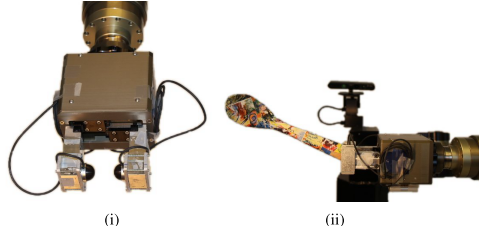
\includegraphics[scale=1]{appendices/pic/5-1}
  \caption*{
  \mtb{图4}在我们的实验评估中,机器人平台的指尖有平行的手爪和光电触觉传感器。}
  \vspace{-0.3cm}
\end{figure}


光学力触觉传感器提供 100Hz 的三轴力测量,
考虑到其低成本、鲁棒性和力控制的适用性,我们选择它们进行实验。
传感器基于光学原理工作,提供 0.03N 的高分辨率力测量,噪声水平约为 0.01N,
这在其他类型的触觉传感器中并不常见。

在我们的实验中,被控物体的惯性和摩擦参数如表一。此外,表二显示了自适
应控制方程(13)和 PI 抓取力控制器(15)中使用的控制器增益和参数。在整个
实验过程中,我们保持控制增益不变。


\begin{table}[!h]
\centering
\caption*{\mtb{表1} 被抓取物体的惯性和摩擦参数}
\begin{tabular}{@{}ccccc@{}}
\toprule[1pt]
\makebox[5em][c]{$I[kg*cm^2]$}  &  \makebox[3em][c]{$m[g]$}  &
\makebox[3em][c]{$l_{cm}[cm]$} &  \makebox[3em][c]{$\mu$}  &
\makebox[3em][c]{$\mu_{tors}$}   \\ \midrule
10.64    & 48.5   &   12.22   &   0.47    & $0.643 \times 10^{-3}$   \\
\bottomrule[1pt]
\end{tabular}
\end{table}


\begin{table}[!h]
\centering
\caption*{\mtb{表2} 用于整个实验的控制器增益和参数}
\begin{tabular}{@{}ccccc@{}}
\toprule[1pt]
\makebox[5em][c]{$k_s$}  &  \makebox[3em][c]{$lambda$}  &
\makebox[3em][c]{$\gamma$} &  \makebox[3em][c]{$k_p$}  &
\makebox[3em][c]{$k_i$}   \\ \midrule
23  &  10.0  &  0.1849  &  $5.0 \times 10^{-4}$  & $2.0 \times 10^{-5}$   \\
\bottomrule[1pt]
\end{tabular}
\end{table}

通过测量机械手手腕上的力/力矩传感器提供的扭转摩擦 $\tau_f$ 和
触觉传感器测量的法向力 $f_n$ ,
我们根据式(5)获得了转动摩擦系数 $\mu_{tors}$ 和幂指数 $\gamma$ 。
然而,由于我们系统的硬件限制,很难准确估计这些参数。
来自力/力矩传感器的摩擦力矩测量具有较低的信噪比,
并且还受到重力补偿误差的影响,从而在估计 $\mu_{tors}$ 的过程中产生较大误差。
我们通过使用不同的摩擦系数运行控制器来调整这个参数,这将在后面进一步解释。

为了获得控制增益,我们首先按照标准 PI 控制器调节方法,
调整抓取力控制器增益 $\left( {{k_p},{k_i}} \right)$ 。
然后通过停用评估机构来调整跟踪控制增益 $k_s$ ,
即在等式(14)中设置 ${\alpha _h} = {\alpha _b} = 0$ ,
并在控制器中使用对象惯性和摩擦参数的真值。过大的跟踪增益 $k_s$ ,
会导致目标进入粘滞状态,沿轨迹运动过程中频繁地停止。
另一方面,较低的 $k_s$ 通常会产生较大的超调量。
我们选择 $\lambda = 10.0$ 作为跟踪控制误差(12),以便给位置跟踪误差提供更高的相对权重,
而不是速度跟踪误差,因为我们的视觉跟踪器的位置估计相对于角速度估计的效果更好。
我们设计的参考轨迹足够慢,以避免运动模糊会降低视觉跟踪器的性能,
尽管较快的速度可以避免粘滞效应。

我们对控制器进行了测试,以评估该控制器在指尖材料的摩擦特性发生改变
时的控制效果,以及在转动摩擦系数 $\mu_{tors}$ 的初始估计值有误差的情况下控制效果。
我们进行了以下一组实验:


\begin{itemize}
	\item 转动摩擦系数 $\mu_{tors}$ 的初值对非自适应控制系统的影响。
    我们停用式(14)中的自适应估计器,实质上是将控制器转换为线性反馈控制器。
    随后我们将展示在控制方程(13)中扭转摩擦系数 $\mu_{tors}$ 的值不同时,
    控制器的控制效果。
	\item 转动摩擦系数 $\mu_{tors}$ 的初值对自适应控制系统的影响。
		我们重复前面的一组实验,并验证自适应控制对于完成旋转任务的重要性。
	\item 改变目标物体的摩擦特征。我们使用与先前实验相同的被控物体,
		但改变其与指尖接触处的材料,即修改摩擦系数,
		进一步检验自适应控制器的性能。
		结果表明,虽然跟踪控制性能明显下降,但目标仍会旋转到目标位置。
\end{itemize}


\appsection{无自适应控制时初始估计误差的影响}

在这组实验中,我们通过在自适应方程(14)中设置
${\alpha _h} = {\alpha _b} = 0.0$ 来停用估计器,
并在控制方程(13)中使用 3 个不同的转动摩擦系数 $\mu_{tors}$ 值来执行控制器。
参考模型的参考轨迹 $\theta_m(t)$ 和物体相对于夹持器的角度 $\theta(t)$ 如图 5 所示。

\begin{figure}[!ht]
  \centering
  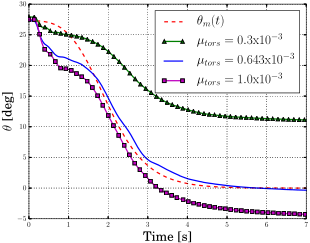
\includegraphics[width=10cm]{appendices/pic/5-2}
  \caption*{
    \mtb{图5} 无自适应控制时,在不同的 $\mu_{tors}$ 值下
    参考位置 $\theta_m$ 和物体的位置 $\theta$ 。}
  \vspace{-0.3cm}
\end{figure}

该实验中我们可以改变使用腕部安装的力矩传感器获得的转动摩擦系数。
在我们的实验测试中,控制器在
${\mu _{tors}} = 0.643 \times {10^{ - 3}}$时获得了最佳的跟踪性能。
此外,当系数低于该最佳值时,例如在图 5 所示的${\mu _{tors}} = 0.3 \times {10^{ - 3}}$时,
物体在到达目标角位置之前过早地停止。
发生这种情况的原因是较低的 $\mu_{tors}$ 使控制方程(13)中的非线
性重力补偿项 $b \tau_g$ 变大,导致控制器施加过大的夹持力。
类似地,高估的扭转摩擦系数,例如 ${\mu _{tors}} = 1.0 \times {10^{ - 3}}$ ,
会减少重力补偿项,并导致物体滑过所需的角度位置。
这个实验清楚地说明了 $\mu_{tors}$ 中的误差如何影响控制性能,
并证明了在我们的方法中使用自适应控制的合理性。


图 6 表示自适应控制器的法向力输入 $u_{f_n}$ ,以及
当 ${\mu _{tors}} = 0.643 \times {10^{ - 3}}$ 时触觉传感器测量的法向力 $f_n$ 。
该图说明力控存在误差,其部分原因可由如图 7 所示的
夹持器内部速度控制器中的跟踪误差来解释,速度跟踪误差表示夹持器速度指令信号
$u_v$ 和通过编码器反馈测量的夹持器速度 $v$ 之间的差异。
这在实际中发生是因为内部控制器的跟踪性能在低速时下降。
我们可以通过使用更灵敏的 PI 力控制器来减少部分力控制误差,
但实际上这会导致物体进入粘滞状态并滞后于参考轨迹。

\begin{figure}[!ht]
  \centering
  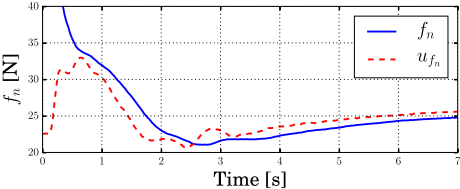
\includegraphics[width=10cm]{appendices/pic/5-3}
  \caption*{
    \mtb{图6}${\mu _{tors}} = 0.643 \times {10^{ - 3}}$时,
    夹持力控制信号 $u_{f_n}$ 和测量的法向力 $f_n$ 。}
  \vspace{-0.3cm}
\end{figure}

\begin{figure}[!ht]
  \centering
  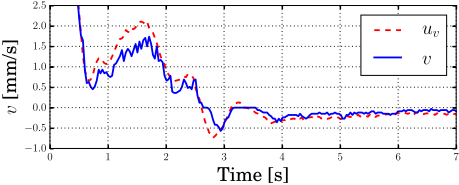
\includegraphics[width=10cm]{appendices/pic/5-4}
  \caption*{
    \mtb{图7}${\mu _{tors}} = 0.643 \times {10^{ - 3}}$时,
    夹持器速度的设定值 $u_v$ 和夹持器速度 $v$ 。}
  \vspace{-0.3cm}
\end{figure}


\appsection{使用自适应控制时初始估计误差的影响}

我们分别将(14a)和(14b)的自适应增益调整为 ${\alpha _h} = 1.5$ 和
${\alpha _b} = 7.5 \times {10^3}$ ,并重复了之前的一组实验,
以分析使用调参律时控制器的性能。
图 8 展示了在保持控制器和自适应增益固定的同时,
具有不同的 $\mu_{tors}$ 的初值的被控物体的角度变化曲线。

\begin{figure}[!ht]
  \centering
  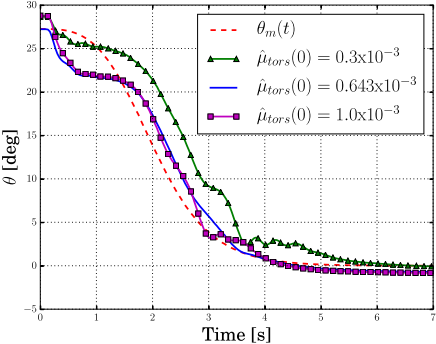
\includegraphics[width=10cm]{appendices/pic/5-5}
  \caption*{
    \mtb{图8}使用自适应估计器时,在 $\mu_{tors}$ 的不同初始估计下,
    目标的参考角位置 $\theta_m$ 和角位置 $\theta$ 。}
  \vspace{-0.3cm}
\end{figure}


我们观察到,
当从正确的扭转摩擦系数估计值 ${\mu _{tors}} = 0.643 \times {10^{ - 3}}$ 开始时,
自适应控制器获得最佳性能。
此外,与先前的一组实验相比,控制器成功地在
低估$({\hat \mu _{tors}}(0) = 0.3 \times {10^{ - 3}})$ 和
高估 $({\hat \mu _{tors}}(0) = 1.0 \times {10^{ - 3}})$ 转动摩擦系数的情况下
收敛到期望角度 $\theta_d$ 。在上述情况下,稳态误差均小于 1 度。

图 9 和 10 示出了当
${\hat \mu _{tors}}(0) = 0.3 \times {10^{ - 3}}$ 时对系统的控制输入。
仍然出现了力控误差。
如前所述,自适应估计不保证收敛到真值,并且图 11 证实了这一点。
该图显示了转动摩擦系数的估算值为 ${\hat \mu _{tors}}(0) = 0.5{\hat b^{ - 1}}$ ,
并未达到其真值。


\appsection{改变物体的摩擦特征}

在这最后一组实验中,我们用摩擦系数较低的材料 $\mu = 0.37$
和摩擦系数较高的材料 $\mu = 1.08$ 替换了被操纵物体的材料 ( $\mu = 0.47$) 。
我们保持控制器和适应增益不变再次进行实验。
实验结果如图 12 和图 13 所示。
与以往的实验相比,虽然自适应控制器的跟踪性能较差,
但稳态误差分别在 1.64 度和 0.5 度内,仍能收敛到期望的目标方向。

\begin{figure}[!ht]
  \centering
  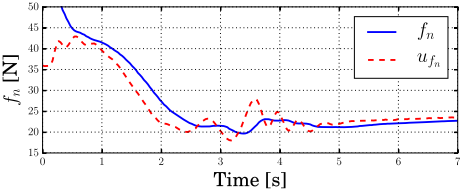
\includegraphics[width=10cm]{appendices/pic/5-6}
  \caption*{
    \mtb{图9}夹持力控制输入 $u_{f_n}$ ,
    使用自适应控制和 $\mu^{tors}(0) = 0.3 \times 10^{−3}$ 时测量法向力 $f_n$ 。}
  \vspace{-0.3cm}
\end{figure}


\begin{figure}[!ht]
  \centering
  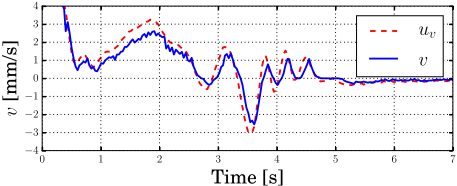
\includegraphics[width=10cm]{appendices/pic/5-7}
  \caption*{
    \mtb{图10}使用自适应控制和 $\hat \mu^{tors}(0) = 0.3 \times 10^{−3}$ 时的
		夹持器速度设定值 $u_v$ 和夹持器速度 $v$ 。}
  \vspace{-0.3cm}
\end{figure}


\begin{figure}[!ht]
	\centering
	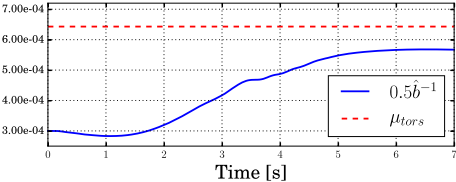
\includegraphics[width=10cm]{appendices/pic/5-8}
	\caption*{
    \mtb{图11} 扭转摩擦系数的自适应估计值 $\mu^{tors} = 0.5 \hat b^{−1}$ 。}
	\vspace{-0.3cm}
\end{figure}


\begin{figure}[!ht]
  \centering
  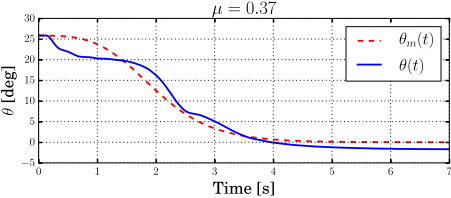
\includegraphics[width=10cm]{appendices/pic/5-9}
  \caption*{
    \mtb{图12}使用 $\mu= 0.37$ 的新材料时物体的角位置 $\theta$。}
  \vspace{-0.3cm}
\end{figure}


\begin{figure}[!ht]
  \centering
  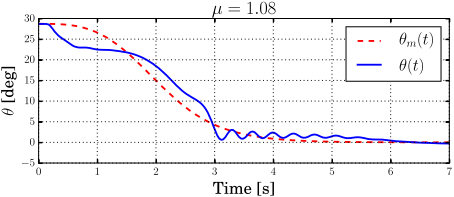
\includegraphics[width=10cm]{appendices/pic/5-10}
  \caption*{
    \mtb{图13}使用 $\mu= 1.08$ 的新材料时物体的角位置 $\theta$。}
  \vspace{-0.3cm}
\end{figure}


\appchapter{结论和工作展望}

提出了一种利用重力和可控滑移实现具有外部灵巧度的旋转运动的自适应控制方法。
考虑到错误估计的摩擦系数是在手操作中常见的误差来源,
我们设计了一种考虑转动摩擦系数误差的自适应控制器。
在我们的控制器中,我们使用视觉跟踪系统测量物体相对于机器人手的位置,
用高分辨率和低噪声的触觉传感器测量物体受到的正压力。
实验结果表明,不准确的转动摩擦系数会对线性反馈控制器的性能会产生显著的负面影响,
然而我们提出的自适应律补偿了这一参数误差并成功地实现了旋转。
由于采用了闭环反馈控制和触觉传感技术,
我们的方法补充了近年来关于内、外灵巧操作的研究成果。

我们工作的一个限制是,我们通过保持夹持器静止来执行被动旋转,
这限制了再抓取的应用范围,除非我们首先旋转夹持器到特定位置。
我们可以通过加速机械臂来扩展该方法,重新设计自适应控制器以抵消惯性力产生的干扰。
我们还可以扩展我们的方法,包括对外部接触的抓握推动,
这就为被抓取物体在机器人手上产生平移运动提供了可能。


\vspace{12bp}
\centerline{\heiti\zihao{-2}\bfseries
  致谢
  \vspace{8bp}
}

这项工作得到了欧盟 FP7 项目 RoboHow.Cog(FP7-ICT-288533)、瑞典研究理
事会(VR)和瑞典战略研究基金会(SSF)的支持。作者衷心感谢大家的支持。作
者还想感谢卡罗莱纳·卢雷罗测试了光电传感器并为其实现了 ROS 软件。


